\section{Policy-Hidden Outsourced ABE}

\begin{figure}
	\centering
	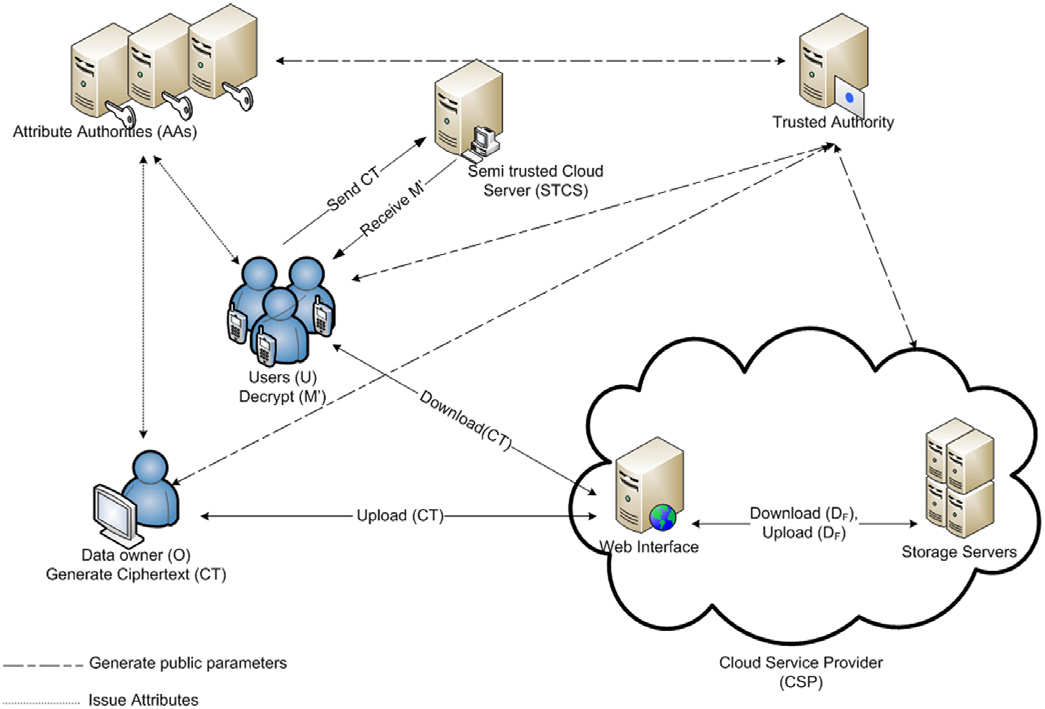
\includegraphics[width=0.8\textwidth]{phoabe-architecture}
	\caption{Architektur von PHOABE \cite{phoabe}}
\end{figure}

Es wird nun ein Überblick zu \textit{PHOABE} (Policy-Hidden Outsourced
Attribute Based Encryption) gegeben, einem Schema, welches aufgrund seiner
Architektur für attribut-basierte Verschlüsselung auf IoT-Geräten interessant
ist. Wie der Name bereits andeutet, handelt es sich hierbei um ein Schema,
welches die Geheimhaltung der Privatsphäre durch Zugriffsstrukturen
gewährleistet (Policy-Hidden). Zudem wird ein STCS verwendet, um den
Entschlüsselungsprozess teilweise auszulagern (Outsourced). Der Grund hierfür
ist, dass IoT-Geräte oft leistungsschwach sind und die Entschlüsselung
hingegen sehr kostspielig ist, weshalb viele andere ABE-Schemata nicht
praktikabel sind. Da ein STCS verwendet wird, stellt PHOABE zudem sicher, dass
die Integrität der Informationen gewährleistet ist. Der Grund für die
Sicherstellung ist, dass angenommen wird, dass der Server selbst korrupt sein
und versuchen könnte, private Daten auszuspähen, uns jedoch trotzdem valide
Ergebnisse erzeugt. Kurz zusammengefasst weist PHOABE folgende Eigenschaften
auf.

\FloatBarrier
\begin{itemize}
	\item Ausgelagert: Die Entschlüsselung wird teilweise durch einen Server
		(STCS) übernommen.
	\item Vertraulichkeit: Eine Änderung des Geheimtextes bewirkt keine
		sinnvolle Änderung der verschlüsselten Nachricht.
	\item Integrität: Es kann überprüft werden, ob die Resultate des STCS
		ge\-fälscht wurden.
	\item Geheimhaltung der Privatsphäre: Zugriffsstrukturen garantieren die
		Sicherung der Privatsphäre.
\end{itemize}

\subsection{Algorithmen}
PHOABE besteht aus insgesamt sieben Algorithmen \cite{phoabe}. Es werden
folgende Symbole für die Darstellung der Komponenten des Schemas verwendet.

\begin{enumerate}
	\item \algitem{Setup}{}{\lambda}{PP} Der
		Setup-Algorithmus nimmt als Eingabe einen Sicherheitsparameter $\lambda$,
		liefert die öffentlichen Parameter $\text{PP}$ und wird von einer
		\textit{Central Trusted Authority} (CTA) ausgeführt.
		\begin{enumerate}
			\item Definition der multiplikativen Gruppen $\mathbb{G}_1$,
				$\mathbb{G}_T$ der Ordnung $p$
			\item Definieren der bilinearen Abbildung $e: \mathbb{G}_1 \times
				\mathbb{G}_1 \to \mathbb{G}_T$ 
			\item Setzen des Generators $g$, sodass $\langle g \rangle = \mathbb{G}_1$
			\item Definieren der Hashfunktion $H' : \left\{ 0,1 \right\}^* \to
				\mathbb{Z}_p$
			\item Definieren der Hashfunktion $H_0 : \left\{ M \right\} \to
				\left\{ 0,1 \right\}^{n_{H_0}}$
			\item Definieren der Hashfunktion $H_1 : \left\{ M \right\} \to
				\left\{ 0,1 \right\}^*$
			\item Definieren der Hashfunktion $H_2 : \left\{ 0,1 \right\}^* \to
				\left\{ 0,1 \right\}^{n_{H_2}}$
			\item \textbf{return} $\left( \mathbb{G}_1, \mathbb{G}_T, p, H', H_0, H_1,
				H_2, e, g\right)$
		\end{enumerate}

	\item \algitem{Setup}{auth}{PP}{\left(sk_{AA_j}, pk_{AA_j}\right)} Bei $N$
		Autoritäten führt die Autorität $AA_j$ mit $j \in N$ diesen Algorithmus
		aus, um einen geheimen Schlüssel $sk_{AA_j}$ und einen öffentlichen
		Schlüssel $pk_{AA_j}$ zu generieren. Als Eingabe nimmt der Algorithmus die
		öffentlichen Umgebungsparameter $PP$.
		\begin{enumerate}
			\item Wähle zwei zufällige Zahlen $\alpha_i, t_i \in \mathbb{Z}^*_N$ für
				jedes Attribut $i$
			\item Wähle eine zufällige Zahl $y \in \mathbb{Z}^*_N$
			\item Berechne den geheimen Schlüssel $sk_{AA_j} = \left(
				\left\{\alpha_i, t_i\right\}, y \right)$
			\item Berechne den öffentlichen Schlüssel $pk_{AA_j} = \left(
				\left\{ e(g, g)^{\alpha_i}, g^{t_i} \right\}, g^y \right)$ 
			\item \textbf{return} $\left( sk_{AA_j}, pk_{AA_j} \right)$
		\end{enumerate}

	\item \algitem{Encrypt}{}{PP, M_{pk}, m, \Phi}{C} Dieser Algorithmus
		ver\-schlüs\-selt die Nachricht $m$ unter Angabe einer Menge der
		öffent\-lich\-en Schlüssel $M_{pk} = \left\{ pk_{AA_j} \;\vert\; j \in N
			\right\}$ und wird vom Datenbesitzer ausgeführt. Jeder dieser Schlüssel
			werden von einer \textit{Attribute Authority} bereitgestellt. Zudem wird
			eine Zugriffsregel $\Phi = \left( A, \rho \right)$ verwendet. Als Ausgabe
			wird ein Geheimtext $C$ erzeugt.
		\begin{enumerate}
			\item Wähle eine zufällige Zahl $a \in \mathbb{Z}^*_N$
			\item Berechne für jedes Attribute den Wert $q_i = e((g^y)^a, H'(x_i))$,
				wobei $x_i \in \Phi$ ein Attribut
				aus der Zugriffsstruktur $\Phi$ ist.
			\item Konvertiere $\Phi$ mithilfe $\left\{q_i\right\}_{i \in F}$ in eine
				LSSS-Matrix $\left( A^{n \times l}, \rho \right)$, wobei $F$ die Anzahl
				der Attribute ist.
			\item Wähle eine zufällige Zahl $s \in \mathbb{Z}_N$.
			\item Wähle $\left\{ p_i \;\vert\; p_i \in \mathbb{Z}^*_N, 0 \leq i \le F
				\right\}$, wobei $F$ die Anzahl der Attribute bzw. Zeilen der
				LSSS-Matrix ist.
			\item Wähle eine zufällige Nachricht $R \in \mathbb{G}_T$ aus der
				Zielgruppe.
			\item Berechne $\lambda_i, \omega_i$ sodass $\lambda_i = \vec{A_i} \cdot
				\vec{v}$ und $\omega_i = \vec{A_i} \cdot \vec{\tau}$, wobei $\vec{v} =
				\left( s, v_1, ..., v_l \right) \in \mathbb{Z}^l_N$ und $\vec{\tau} =
				\left( 0, \tau_1, ... \tau_l \right) \in \mathbb{Z}^l_N$ zwei zufällige
				Vektoren aus dem $l$-dimensionalen Raum von $\mathbb{Z}_N$ sind.
			\item 
		\end{enumerate}

	\item\label{enum:phoabe_keygen} \algitem{Keygen}{}{PP, sk_{AA_j}, pk_{AA_j},
		GID, S_{j, GID}}{sk_{j, GID}} Dieser Algorithmus erzeugt einen privaten
		Schlüssel $sk_{j, GID}$ und wird von einer \textit{Attribute Authority}
		$AA_j$ ausgeführt. Der Schlüssel wird für einen Benutzer erzeugt und steht
		in Verbindung mit den Attributen $S_{j, GID} = \left\{ a_1, ..., a_{n_j}
		\right\}$ der $AA_j$.  Dabei stellt $a \in S_{j, GID}$ ein Attribut und
		$n_j$ die Anzahl der Attribute von $AA_j$ dar. $GID$ ist die Identität vom
		Benutzer.

	\item \algitem{Transform}{}{PP, M_{sk}, p, C}{M_{tk}} Dieser Algorithmus
		wird von einem Benutzer ausgeführt. Dieser besitzt eine Menge von
		Attributen $S_{GID}$ und die dazugehörigen Schlüssel $M_{sk} = \left\{
		sk_{j, GID} \;\vert\; j \in N \right\}$. Die Schlüssel wurden vorher durch
		\textit{Attribute Authorities} für den Benutzer ausgestellt (siehe Punkt
		\ref{enum:phoabe_keygen}). Als Eingabe nimmt der Algorithmus zusätzlich
		die öffentlichen Parameter $PP$, die Zugriffsregel $p = \left(A,
		\rho\right)$ und den Geheimtext $C$. Als Ausgabe wird eine Menge von
		transformierten Schlüsseln $M_{tk} = \left( \left\{tpk_{j, GID} \;\vert\;
		j \in N\right\}, tsk_{GID} \right)$ erzeugt.

	\item \algitem{Decrypt}{out}{PP, M_{tk}, p, C}{m'} Dieser Algorithmus wird
		vom STCS ausgeführt und erzeugt die teilweise entschlüsselte Nachricht
		$m'$. Als Eingabe nimmt der Algorithmus die öffentlichen Parameter $PP$,
		eine Menge von transformierten Schlüsseln $M_tk$, die Zugriffsregeln $p =
		\left(A, \rho\right)$ und den Geheimtext $C$.

	\item \algitem{Decrypt}{}{m', tks_{GID}}{m} Dieser Algorithmus wird von
		Benutzer ausgeführt und nimmt als Eingabe die teilweise entschlüsselte
		Nachricht $m'$ und den geheimen Transformationsschlüssel $tsk_{GID}$. Als
		Ausgabe wird die Nachricht $m$ erzeugt.
\end{enumerate}

\begin{center}
\begin{small}
	\begin{tabular}{p{3cm}p{9cm}}
		\hline
		Symbol & Beschreibung \\
		\hline
		STCS & Semi Trusted Cloud Server \\
		CTA & Central Trusted Authority \\
		$\lambda$ & Sicherheitsparameter \\
		$AA_j$ & Die $j$-te Attribute Authority \\
		$PP$ & Public Parameter \\
		$sk_{AA_j}$ & Der geheime Schlüssel der $j$-ten Attribute Authority \\
		$pk_{AA_j}$ & Der öffentliche Schlüssel der $j$-ten Attribute Authority \\
		$M_{pk}$ & Menge der öffentlichen Schlüssel aller Attribute Authorities \\
		$A$ & Zugriffsstruktur in LSSS-Matrix-Darstellung \\
		$\rho$ & Abbildung zum Auslesen einer Zeile von $A$ \\
		$\Phi$ & Die Zugriffsregeln bestehend aus $\Phi = \left(A, \rho\right)$ \\
		$C$ & Der aus der Nachricht erzeugte Geheimtext \\
		$GID$ & Die Identität eines Benutzers \\
		$S_{j, GID}$ & Menge von Attributen der $j$-ten Attibute Authority für den
		Benutzer mit der Identität $GID$ \\
		$sk_{j, GID}$ & Der geheime Schlüssel der $j$-ten Attribute Authority für
		den Benutzer mit der Identität $GID$ \\
		$M_{sk}$ & Menge von geheimen Schlüsseln $sk_{j, GID}$ der $j$-ten Attribute
		Authority \\
		$M_{tk}$ & Menge der Transformationsschlüssel $tk_{j, GID} \in M_{tk}$ \\
		$tpk_{j, GID}$ & Öffentlicher Transformationsschlüssel der $j$-ten
		Attribute Authority für den Benutzer mit der Identität $GID$ \\
		$tsk_{j, GID}$ & Geheimer Transformationsschlüssel der $j$-ten
		Attribute Authority für den Benutzer mit der Identität $GID$ \\
		$m$ & Die Nachricht \\
		$m'$ & Die teilweise entschlüsselte Nachricht vom STCS \\
		\hline
	\end{tabular}
\end{small}
\end{center}
